% ===================================================================
\chapter{Compression Methods}
\label{ch:methods}

This chapter describes the methods compared in this thesis. It starts with the
eight candidates and what each one does, then specifies in detail the two that
were taken to hardware: the entropy coder they share, the axis along which they
predict, the two predictors themselves, and the Huffman dictionary that turns
their prediction errors into bits.

\section{The eight candidate methods}
\label{sec:candidates}

Every method operates on the same input: the range-FFT output of each frame,
quantised to 16-bit integers by the FX16 step of Section~\ref{sec:fx16}, except
where a method replaces that step. All eight were implemented in the same
MATLAB chain and scored with the same metrics (Chapter~\ref{ch:evaluation}).

\begin{description}[leftmargin=!,labelwidth=26mm,style=nextline,font=\normalfont\bfseries]
\item[FP16, FX16] The two reference formats, as in Kiem's thesis: 16-bit
floating point, and the 16-bit integer codes of the FX16 step. Neither
compresses; FX16 is the input to every integer method below, so its detection
losses are the floor that any of them can reach.
\item[BAQ] Block adaptive quantisation, implemented in block-floating-point
form: each block of 16 range bins shares an 8-bit exponent chosen from the
block maximum, and each real and imaginary part keeps a 4-bit mantissa, so the
ratio is fixed at $32/(8 + 8/16) = 3.76$. It stands in for the
block-floating-point family (NXP's CP4/CP8 and Infineon's CMPRA/CMPRB are of
the same kind) and for BAQ proper \cite{kwok1989}. Lossy.
\item[RDVLE] Range-dependent variable-length encoding \cite{li2014}: fewer
bits for far range bins, following the fall of received power with range, here
capped at three bits removed. Lossy.
\item[RDVLE+UDRE] RDVLE followed by uniform dynamic-range re-encoding of
blocks of 16 bins at six bits \cite{li2014}. Lossy.
\item[DRHE] Doppler Redundancy Hybrid Encoding, as specified by Kiem
(Section~\ref{sec:drhe}): slow-time prediction in polar form, followed by the
entropy coder of Section~\ref{sec:entropycoder}. Lossless with respect to the
FX16 codes.
\item[DRHE fp16] The same predictor applied to FP16 values instead of FX16
codes, to test whether floating-point storage --- the remedy Kiem suggested for
quantisation error --- can be compressed.
\item[LPC] A second-order linear predictive coder designed for this thesis
(Section~\ref{sec:lpc}). It predicts along the same axis as DRHE and uses the
same entropy coder, so that only the predictor differs. Lossless with respect
to the FX16 codes.
\end{description}

\noindent
NXP's formats were not implemented separately, since their exact bit layouts
are proprietary and the block-floating-point quantiser represents the family.
Neural and spectral methods such as AdaRadar \cite{park2026} were left out of
scope: they are lossy, and their decoders run on the central processor.

The rest of this chapter concerns DRHE and LPC, which Section~\ref{sec:stage1}
shows are the only two methods that compress by more than three without losing
detections.

\section{The shared entropy coder: turning residuals into bits}
\label{sec:entropycoder}

This section is deliberately detailed. The entropy coder is where the
compression ratio is physically realised --- it is the only part of either
design that actually emits bits --- so understanding exactly what it charges
for is what makes the results of Chapter~\ref{ch:results} interpretable rather
than merely quotable. Both predictive compressors in this thesis use exactly
this coder.

\subsection{What a residual is}
\label{sec:whatresidual}

Let $x[m]$ be the sample to be transmitted and let $P$ be some rule --- the
\emph{predictor} --- that produces an estimate
\begin{equation}
\hat{x}[m] = P\bigl(x[m-L],\, x[m-2L],\, \ldots\bigr)
\end{equation}
from samples that have \emph{already been transmitted}. The encoder does not
send $x[m]$. It sends the \emph{residual}
\begin{equation}
\label{eq:residualdef}
d[m] = x[m] - \hat{x}[m].
\end{equation}

The decoder, having already reconstructed $x[m-1], x[m-2], \ldots$, runs the
identical rule $P$ on them, obtains the identical $\hat{x}[m]$, and recovers
\begin{equation}
x[m] = d[m] + \hat{x}[m].
\end{equation}
The lag $L$ is the distance back along the ramp axis to the samples used for
prediction; Section~\ref{sec:predaxis} explains why it is $L = \nTx = 12$ on
this radar rather than $1$.

Two things follow, and both matter.

\paragraph{Nothing is lost.}
Equation~\eqref{eq:residualdef} is a \emph{re-expression}, not an
approximation. Given $\hat{x}[m]$, the map $x \mapsto d$ is a bijection. The
sequence $\{d[m]\}$ carries exactly the information the sequence $\{x[m]\}$
carried --- no more, no less. This is why a predictive coder can be lossless at
all.

\paragraph{The predictor must be causal.}
$P$ may only use samples the decoder already has, or side information sent
ahead of them. A predictor that peeked at $x[m]$ itself would be
unreproducible at the far end. It is also why Section~\ref{sec:closedloop}
makes such a point of \emph{which} version of the past the encoder uses ---
the originals or the reconstructions --- since those differ the moment anything
is not exactly lossless.

\subsection{Why a re-expression can be worth anything}

If no information is lost and none is gained, why is the residual sequence any
cheaper to write down?

Because the \emph{distribution} has changed, and a well-chosen code charges by
distribution. Table~\ref{tab:rawvsresid} shows this on real data: one range bin
of one receive channel, sixteen consecutive ramps, taken from frame~0 of the
ColoRadar capture, predicted twelve ramps back by DRHE.

\begin{table}[t]
\centering
\caption[Raw values against residuals]{The same sixteen real samples, written
two ways. Range bin 75, receive channel 1, ramps 168--183. Both rows carry
identical information.}
\label{tab:rawvsresid}
\small
\setlength{\tabcolsep}{3.4pt}
\begin{tabular}{@{}l*{16}{r}@{}}
\toprule
$m$ & 168 & 169 & 170 & 171 & 172 & 173 & 174 & 175 & 176 & 177 & 178 & 179 & 180 & 181 & 182 & 183\\
\midrule
$x$ (raw) & $-69$ & $-52$ & $59$ & $-6$ & $-29$ & $-15$ & $59$ & $-20$ & $-69$ & $-73$ & $-45$ & $84$ & $-73$ & $-50$ & $59$ & $-5$\\
$d$ (residual) & $3$ & $-3$ & $0$ & $-1$ & $1$ & $3$ & $-4$ & $3$ & $-1$ & $-2$ & $-1$ & $0$ & $-2$ & $4$ & $-1$ & $1$\\
\bottomrule
\end{tabular}
\end{table}

The raw values swing over $[-73, +84]$; writing any of them needs eight bits.
The residuals never leave $[-4, +4]$; four bits would do. Since the two rows
are informationally equivalent, that factor of two is free --- provided the
coder can be told about it.

And there is the catch. The bound $[-4,+4]$ holds for \emph{these} sixteen
samples. Somewhere else in the frame a target appears, or the scene changes,
and a residual of $400$ arrives. A fixed four-bit field cannot carry it. What
is needed is a code that spends few bits on the common case, many on the rare
one, and lets the decoder tell which is which.

\subsection{The parsing problem}

The naive approach fails immediately. Suppose the rule were ``small values get
four bits, large values get twelve''. When the decoder reads four bits, it has
no way to know whether it has just read a complete small value or the first
third of a large one. Variable-length coding is not merely a matter of writing
fewer bits; it is a matter of writing them so that the boundaries can be
recovered.

There are two standard answers:

\begin{enumerate}
\item \textbf{A prefix-free code over every possible value.} Assign every one
of the \num{65536} possible 16-bit residuals its own codeword, no codeword
being a prefix of another. This is optimal, and it is what a Huffman code over
the raw alphabet would give --- but it needs a \num{65536}-entry table, and the
table has to be derived from the data and transmitted alongside it.

\item \textbf{Split the value into a size and a payload.} Send a small
\emph{description of how big the value is}, coded with a prefix-free code over
a handful of symbols, followed by the value itself in exactly that many raw
bits. The decoder reads the size first, so it always knows how many bits to
read next.
\end{enumerate}

Both compressors here take the second route, which is the same construction
JPEG uses for DC coefficients. It is cheap in every respect that matters for
hardware: the prefix-free table has sixteen entries rather than \num{65536}, it
can be fixed at design time rather than derived per frame, and decoding a
symbol is a sixteen-way comparison rather than a tree walk.

\subsection{The category $S_4$}

The ``size'' half of the split is the category
\begin{equation}
\label{eq:s4}
S_4(v) =
\begin{cases}
0 & v = 0,\\[2pt]
\min\bigl(15,\ \lfloor \log_2 |v| \rfloor + 1\bigr) & v \neq 0,
\end{cases}
\end{equation}
which is simply the number of bits needed to write $|v|$. Its ranges are given
in Table~\ref{tab:catranges}.

\begin{table}[h]
\centering
\caption[S4 category ranges]{The first few categories. Category $k \geq 1$
covers $|v| \in [2^{k-1},\, 2^k - 1]$, which counting both signs is exactly
$2^k$ distinct values --- precisely what $k$ raw bits can enumerate.}
\label{tab:catranges}
\small
\begin{tabular}{@{}rlrl@{}}
\toprule
$S_4$ & values covered & count & \\
\midrule
0 & $v = 0$ & 1 & the only category with no payload\\
1 & $v \in \{-1, +1\}$ & 2 & \\
2 & $|v| \in \{2,3\}$ & 4 & \\
3 & $|v| \in [4,7]$ & 8 & \\
4 & $|v| \in [8,15]$ & 16 & \\
$\vdots$ & & & \\
15 & $|v| \in [16384, 32767]$ & \num{32768} & exactly fills 15 bits\\
\bottomrule
\end{tabular}
\end{table}

The design is tight by construction: category $k$ contains exactly $2^k$
values, so $k$ payload bits identify one of them with nothing wasted and
nothing left over. Section~\ref{sec:robust} deals with the one value for which
``nothing left over'' becomes a problem.

\subsection{The APPEND bits}

The payload half is
\begin{equation}
\label{eq:append}
A(v) =
\begin{cases}
v & v \geq 0,\\
v + 2^{S_4(v)} - 1 & v < 0,
\end{cases}
\end{equation}
written in $S_4(v)$ raw bits.

The offset for negative values looks arbitrary but is doing something specific.
Table~\ref{tab:cat3} enumerates category~3 in full.

\begin{table}[h]
\centering
\caption[Category 3 enumerated]{Every codepoint of category 3. The negative
values map to patterns with a clear most significant bit, the positive values
to patterns with it set --- so the sign is recovered from that one bit without
transmitting a sign bit.}
\label{tab:cat3}
\small
\begin{tabular}{@{}rrlc@{}}
\toprule
$v$ & $A(v)$ & 3-bit pattern & MSB \\
\midrule
$-7$ & 0 & \texttt{000} & 0\\
$-6$ & 1 & \texttt{001} & 0\\
$-5$ & 2 & \texttt{010} & 0\\
$-4$ & 3 & \texttt{011} & 0\\
$+4$ & 4 & \texttt{100} & 1\\
$+5$ & 5 & \texttt{101} & 1\\
$+6$ & 6 & \texttt{110} & 1\\
$+7$ & 7 & \texttt{111} & 1\\
\bottomrule
\end{tabular}
\end{table}

Because positive values in category $k$ span $[2^{k-1}, 2^k - 1]$ --- exactly
the $k$-bit patterns with the top bit set --- and the offset maps the negatives
onto $[0, 2^{k-1} - 1]$ --- exactly those with it clear --- the sign falls out
of the payload for free. The decoder's rule is therefore
\begin{equation}
v = \begin{cases}
A & \text{if the MSB of the $S_4$ payload bits is set},\\
A - \bigl(2^{S_4} - 1\bigr) & \text{otherwise},
\end{cases}
\end{equation}
which in hardware is one bit test and one subtract.

\subsection{Cost, and the shape of the dictionary}
\label{sec:huffman}

The total cost of coding one residual is
\begin{equation}
\label{eq:cost}
L(v) = \underbrace{\ell\bigl(S_4(v)\bigr)}_{\text{Huffman codeword}}
     + \underbrace{S_4(v)}_{\text{payload}},
\end{equation}
where $\ell(\cdot)$ is the codeword length for that category. The dictionary is
\emph{fixed} --- not computed per frame --- which saves transmitting it and
removes a serial dependency from the hardware. The \emph{original} dictionary,
taken from Kiem's thesis, has lengths
\begin{equation}
\ell = [\,4,3,2,2,2,5,6,7,8,9,10,11,14,14,13,12\,]\ \text{bits}.
\end{equation}
The full dictionary, codewords included, is in Appendix~\ref{app:huffman}.
Every one of the sixteen entries was verified against the published table
\cite[Table~A.1]{kiem2025}; all sixteen agree once the published
most-significant-bit-first codes are reversed for the least-significant-bit-first
packer used in this implementation.

Substituting into Equation~\eqref{eq:cost} gives the cost curve of the original
dictionary:

\begin{table}[h]
\centering
\small
\begin{tabular}{@{}rrrrr@{}}
\toprule
$S_4$ & $|v|$ range & $\ell$ & payload & \textbf{total} \\
\midrule
0 & $0$        & 4 & 0 & \textbf{4}\\
1 & $1$        & 3 & 1 & \textbf{4}\\
2 & $2$--$3$   & 2 & 2 & \textbf{4}\\
3 & $4$--$7$   & 2 & 3 & \textbf{5}\\
4 & $8$--$15$  & 2 & 4 & \textbf{6}\\
5 & $16$--$31$ & 5 & 5 & \textbf{10}\\
6 & $32$--$63$ & 6 & 6 & \textbf{12}\\
7 & $64$--$127$& 7 & 7 & \textbf{14}\\
8 & $128$--$255$& 8 & 8 & \textbf{16}\\
\bottomrule
\end{tabular}
\end{table}

Three features of this curve deserve attention.

\paragraph{Everything below 16 is nearly free.}
A residual anywhere in $[-15, +15]$ costs between four and six bits. Against
sixteen raw bits that is already a compression ratio between \num{2.7} and
\num{4.0}, achieved without the predictor doing anything clever --- it only has
to keep residuals small.

\paragraph{There is a cliff at category 5.}
Cost jumps from six bits to ten. A residual of \num{15} costs six bits; a
residual of \num{16} costs ten. The coder is, by design, forgiving of small
errors and severe about larger ones.

\paragraph{Above category 8 the code loses.}
A residual of \num{128} costs sixteen bits --- exactly what the raw value
would have cost. Beyond that the coder actively expands. This is not a flaw:
it is the inevitable consequence of assigning short codewords to some symbols,
and it is why the \texttt{random-int16} edge case of
Section~\ref{sec:edgecases} expands the data by \SI{67}{\percent}.

The dictionary's shape encodes an assumption about the data --- that categories
2, 3 and 4 dominate, since those get the two-bit codewords --- and it can never
code a value in fewer than four bits. Section~\ref{sec:dict} shows that the
prediction errors of this thesis are smaller than that, and derives
dictionaries that match them.

\subsection{Worked example 1: one value, in full}

Take $v = -5$.

\begin{enumerate}
\item $|v| = 5$, and $\lfloor \log_2 5 \rfloor + 1 = 3$, so $S_4 = 3$.
\item $v < 0$, so $A(v) = -5 + 2^3 - 1 = 2$, written in three bits as
\texttt{010}.
\item The original dictionary gives category 3 the codeword \texttt{00}, two
bits.
\item The emitted bits are \texttt{00}\,\texttt{010} --- five bits, against
sixteen for the raw value.
\end{enumerate}

Decoding runs the same steps backwards. The decoder matches \texttt{00} against
the dictionary, recovers $S_4 = 3$, reads the next three bits \texttt{010},
sees the most significant is \texttt{0} so the value was negative, and computes
$2 - (2^3 - 1) = -5$.

\section{Predicting on a time-division MIMO radar}
\label{sec:predaxis}

Both predictors work along \emph{slow time}: they predict a range bin's value
in one ramp from its values in earlier ramps. Section~\ref{sec:tdm} showed that
on a TDM-MIMO cascade the ramp axis interleaves the transmitters, so ramp $m$
and ramp $m-1$ come from different antennas eleven times in twelve. The two
predictors are therefore applied at a lag of $L = \nTx = 12$ ramps: each ramp
is predicted from the previous ramp of the \emph{same} transmitter. This
section shows on real data why that choice matters.

Table~\ref{tab:worked16} traces sixteen consecutive ramps of one range bin ---
the same bin as Table~\ref{tab:rawvsresid} --- through the DRHE predictor twice.
The left half predicts from ramp $m-1$, which is how slow-time prediction is
described for a single-transmitter radar. The right half predicts from ramp
$m - \nTx$. Everything else --- the filters, the coefficients, the entropy
coder, the dictionary --- is identical between the two halves.

\begin{table}[htbp]
\centering
\caption[Sixteen samples traced through both predictors]{Sixteen real samples
traced through DRHE at two prediction lags. Range bin 75, receive channel 1,
frame 0, ramps 168--183; real part shown, the imaginary part behaves
identically. The window is late enough in the frame that both predictors'
filters are fully converged. The two halves differ only in which earlier ramp
the prediction comes from.}
\label{tab:worked16}
\small
\setlength{\tabcolsep}{4pt}
\begin{tabular}{@{}rr r@{\hskip 10pt} rrrr @{\hskip 10pt} rrrr@{}}
\toprule
& & & \multicolumn{4}{c}{\textbf{predicted from ramp $m-1$}}
    & \multicolumn{4}{c}{\textbf{predicted from ramp $m-\nTx$}}\\
\cmidrule(lr){4-7}\cmidrule(lr){8-11}
$m$ & TX & $x$ & $\hat{x}$ & $d$ & $S_4$ & bits & $\hat{x}$ & $d$ & $S_4$ & bits\\
\midrule
168 & 0  & $-69$ & $67$  & $-136$ & 8 & 16 & $-72$ & $3$  & 2 & 4\\
169 & 1  & $-52$ & $-75$ & $23$   & 5 & 10 & $-49$ & $-3$ & 2 & 4\\
170 & 2  & $59$  & $81$  & $-22$  & 5 & 10 & $59$  & $0$  & 0 & 4\\
171 & 3  & $-6$  & $64$  & $-70$  & 7 & 14 & $-5$  & $-1$ & 1 & 4\\
172 & 4  & $-29$ & $24$  & $-53$  & 6 & 12 & $-30$ & $1$  & 1 & 4\\
173 & 5  & $-15$ & $-29$ & $14$   & 4 & 6  & $-18$ & $3$  & 2 & 4\\
174 & 6  & $59$  & $-6$  & $65$   & 7 & 14 & $63$  & $-4$ & 3 & 5\\
175 & 7  & $-20$ & $-83$ & $63$   & 6 & 12 & $-23$ & $3$  & 2 & 4\\
176 & 8  & $-69$ & $-93$ & $24$   & 5 & 10 & $-68$ & $-1$ & 1 & 4\\
177 & 9  & $-73$ & $-65$ & $-8$   & 4 & 6  & $-71$ & $-2$ & 2 & 4\\
178 & 10 & $-45$ & $-44$ & $-1$   & 1 & 4  & $-44$ & $-1$ & 1 & 4\\
179 & 11 & $84$  & $28$  & $56$   & 6 & 12 & $84$  & $0$  & 0 & 4\\
180 & 0  & $-73$ & $70$  & $-143$ & 8 & 16 & $-71$ & $-2$ & 2 & 4\\
181 & 1  & $-50$ & $-75$ & $25$   & 5 & 10 & $-54$ & $4$  & 3 & 5\\
182 & 2  & $59$  & $81$  & $-22$  & 5 & 10 & $60$  & $-1$ & 1 & 4\\
183 & 3  & $-5$  & $67$  & $-72$  & 7 & 14 & $-6$  & $1$  & 1 & 4\\
\midrule
\multicolumn{6}{r}{\textbf{total bits}} & \textbf{176} & & & & \textbf{66}\\
\multicolumn{6}{r}{bits per value} & 11.00 & & & & 4.12\\
\multicolumn{6}{r}{compression ratio} & 1.455 & & & & \textbf{3.879}\\
\bottomrule
\end{tabular}
\end{table}

The left half is a predictor working across the wrong axis. Its residuals ($-136$,
$+23$, $-22$, $-70$, \ldots) are frequently \emph{larger in magnitude than the
samples they replace}, they land in categories 5 through 8, and they cost
\num{11.00} bits per value --- a compression ratio of \num{1.455}, which is to
say the entropy coder is salvaging a little from a predictor that has actively
made things worse.

The right half is the same predictor twelve ramps back. Its residuals never
exceed 4 in magnitude, they land in categories 0 through 3, and they cost
\num{4.12} bits per value.

\begin{figure}[t]
\centering
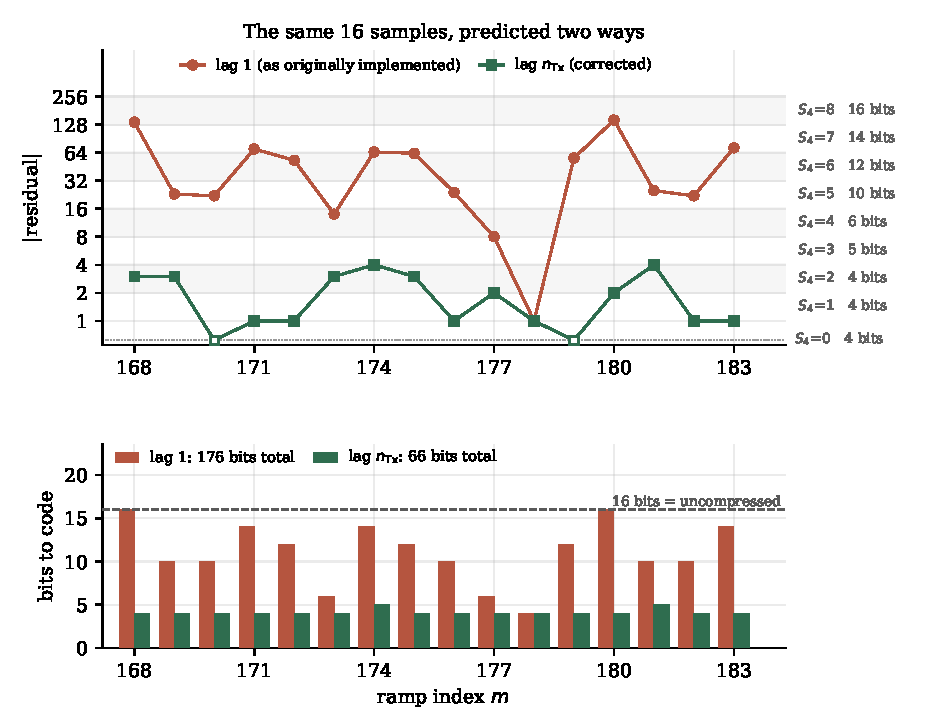
\includegraphics[width=\textwidth]{fig_worked.pdf}
\caption[The sixteen samples, plotted]{Table~\ref{tab:worked16} drawn. Above:
residual magnitude on a logarithmic scale, with the $S_4$ category bands and
their bit costs marked on the right; hollow markers are residuals of exactly
zero. Below: the bits each sample costs, against the \num{16} bits it would
have taken uncompressed. The lag-1 predictor spends \num{176} bits on this
window; the same predictor on the correct axis spends \num{66}.}
\label{fig:worked}
\end{figure}

\subsubsection*{Why the difference is so large}

Table~\ref{tab:workedpolar} answers this directly, and it is worth studying
because it is the mechanism behind the prediction gains reported in
Chapter~\ref{ch:results}.
DRHE (Section~\ref{sec:drhe}) predicts magnitude with a smoother and phase with
a double integrator, both of which work when the quantity being predicted
changes slowly and smoothly.

\begin{table}[t]
\centering
\caption[Why the two lags differ]{The same window in polar coordinates. Against
ramp $m-1$ the magnitude moves by up to \num{22} and the phase jumps
unpredictably over the full $\pm\pi$ range. Against ramp $m-\nTx$ the
magnitude moves by at most \num{4} and the phase increment is essentially zero
--- a stationary target, exactly what the double integrator is built for.}
\label{tab:workedpolar}
\small
\setlength{\tabcolsep}{6pt}
\begin{tabular}{@{}rr rr @{\hskip 12pt} rr @{\hskip 12pt} rr@{}}
\toprule
& & \multicolumn{2}{c}{sample}
  & \multicolumn{2}{c}{change vs.\ $m-1$}
  & \multicolumn{2}{c}{change vs.\ $m-\nTx$}\\
\cmidrule(lr){3-4}\cmidrule(lr){5-6}\cmidrule(lr){7-8}
$m$ & TX & $|x|$ & $\angle x$ & $\Delta|x|$ & $\Delta\theta$ & $\Delta|x|$ & $\Delta\theta$\\
\midrule
168 & 0  & 74.1  & $-2.769$ & $-21.8$ & $-2.244$ & $-3.2$ & $\phantom{-}0.002$\\
169 & 1  & 91.3  & $-2.177$ & $17.2$  & $0.592$  & $-0.0$ & $-0.040$\\
170 & 2  & 101.0 & $-0.947$ & $9.8$   & $1.230$  & $-2.5$ & $\phantom{-}0.017$\\
171 & 3  & 110.2 & $-1.625$ & $9.1$   & $-0.678$ & $3.0$  & $-0.008$\\
172 & 4  & 107.0 & $-1.845$ & $-3.2$  & $-0.220$ & $-2.2$ & $\phantom{-}0.004$\\
173 & 5  & 112.0 & $-1.705$ & $5.0$   & $0.140$  & $-0.3$ & $\phantom{-}0.018$\\
174 & 6  & 97.0  & $0.917$  & $-15.0$ & $2.622$  & $-0.4$ & $\phantom{-}0.023$\\
175 & 7  & 81.5  & $1.819$  & $-15.5$ & $0.902$  & $0.4$  & $-0.027$\\
176 & 8  & 73.4  & $2.794$  & $-8.1$  & $0.975$  & $-0.1$ & $\phantom{-}0.043$\\
177 & 9  & 75.0  & $-2.913$ & $1.6$   & $0.576$  & $2.4$  & $\phantom{-}0.021$\\
178 & 10 & 95.3  & $-2.063$ & $20.3$  & $0.850$  & $0.9$  & $\phantom{-}0.005$\\
179 & 11 & 97.8  & $-0.537$ & $2.5$   & $1.526$  & $1.9$  & $-0.013$\\
180 & 0  & 77.5  & $-2.799$ & $-20.3$ & $-2.263$ & $3.4$  & $-0.031$\\
181 & 1  & 92.6  & $-2.141$ & $15.2$  & $0.659$  & $1.4$  & $\phantom{-}0.036$\\
182 & 2  & 102.6 & $-0.958$ & $10.0$  & $1.182$  & $1.6$  & $-0.011$\\
183 & 3  & 106.1 & $-1.618$ & $3.5$   & $-0.659$ & $-4.0$ & $\phantom{-}0.007$\\
\bottomrule
\end{tabular}
\end{table}

Look at the $\Delta\theta$ columns. Against ramp $m-1$ the phase increment is
$-2.244$, then $+0.592$, then $+1.230$, then $-0.678$ --- it swings over most
of $[-\pi, \pi]$ with no pattern a two-tap filter could follow. Against ramp
$m - \nTx$ it is $0.002$, $-0.040$, $0.017$, $-0.008$: essentially
zero, frame after frame, because this is a stationary target and twelve ramps
later the same antenna sees the same phase.

The magnitude column tells the same story: $\pm 22$ against the immediate
predecessor, $\pm 4$ against the same-transmitter predecessor.

The reason is the one given in Section~\ref{sec:tdm}. Ramps 168 and 167 were
transmitted by \emph{different antennas}, so the phase between them is set by
where the target is in \emph{angle}, via
Equation~\eqref{eq:steering} --- and the twelve transmitters are at twelve
different positions, so that phase jumps around on a period-12 pattern. Ramps
168 and 156 were transmitted by the \emph{same} antenna, so the phase between
them is set by how fast the target is \emph{moving}, via
Equation~\eqref{eq:dopplerphase} --- and it is not moving.

\subsubsection*{The actual bits}

It is worth seeing the bitstream itself. Coding the first six residuals of the
lag-$\nTx$ column, using Equations~\eqref{eq:s4} and~\eqref{eq:append} and the
dictionary of Appendix~\ref{app:huffman}:

\begin{center}
\small
\begin{tabular}{@{}rrrlll r@{}}
\toprule
$d$ & $S_4$ & $A(d)$ & codeword & payload & emitted & bits\\
\midrule
$+3$ & 2 & 3 & \texttt{10}   & \texttt{11}  & \texttt{10\,11}   & 4\\
$-3$ & 2 & 0 & \texttt{10}   & \texttt{00}  & \texttt{10\,00}   & 4\\
$0$  & 0 & --- & \texttt{0101} & ---        & \texttt{0101}     & 4\\
$-1$ & 1 & 0 & \texttt{001}  & \texttt{0}   & \texttt{001\,0}   & 4\\
$+1$ & 1 & 1 & \texttt{001}  & \texttt{1}   & \texttt{001\,1}   & 4\\
$+3$ & 2 & 3 & \texttt{10}   & \texttt{11}  & \texttt{10\,11}   & 4\\
\bottomrule
\end{tabular}
\end{center}

\noindent
which concatenates to the 24-bit stream
\begin{center}
\texttt{1011\,1000\,0101\,0010\,0011\,1011}
\end{center}
carrying six samples that would have occupied \num{96} bits raw. (The
codewords are shown in their stored, bit-reversed form; Appendix~\ref{app:huffman}
lists both forms.)

The same six samples at lag 1 --- residuals $-136$, $+23$,
$-22$, $-70$, $-53$, $+14$ --- fall into categories 8, 5, 5, 7, 6 and 4 and
occupy $16 + 10 + 10 + 14 + 12 + 6 = \num{68}$ bits. Nearly three times as many,
for identical information.


\subsection{Why not one model per transmitter?}

An alternative way to keep prediction on one antenna is to split each frame
into twelve independent 16-ramp blocks, one per transmitter, and predict within
each. For DRHE that is equivalent to the lag-$\nTx$ indexing above. For LPC it
is not: fitting separate coefficients to each block multiplies the side
information by twelve, from \SI{1.04}{\percent} to \SI{12.5}{\percent} of the
uncompressed frame, and shortens each autocorrelation estimate from 192 ramps
to 16, which makes the coefficients much noisier. Measured over five frames it
compresses to only \num{2.63}, worse than not predicting at all. Keeping one
coefficient pair per (bin, channel, part) and moving the lags to $\nTx$ and
$2\nTx$ costs no extra side information, and is the design used here. On a
TDM-MIMO radar the right change is to the \emph{lag}, not to the
\emph{partitioning}.

\section{DRHE: Doppler Redundancy Hybrid Encoding}
\label{sec:drhe}

DRHE \cite{li2014,zivkovic2015} exploits the redundancy of radar data along the
Doppler (slow-time) axis, and is a \emph{hybrid} of prediction and entropy
coding: a predictor removes the slow-time structure, and an entropy coder ---
originally run-length plus Huffman, here the $S_4$ coder of
Section~\ref{sec:entropycoder} --- codes what is left.

\subsection{Why predict in polar coordinates}

Section~\ref{sec:fmcw} established what a range-bin sequence looks like across
slow time for a target at constant velocity: the \emph{magnitude} is nearly
constant, and the \emph{phase} advances by a constant increment. In Cartesian
$(I,Q)$ coordinates that is a point rotating on a circle --- both components
oscillate, and a simple difference between consecutive samples is large. In
polar coordinates the same sequence is two nearly-trivial signals: a constant
and a ramp.

DRHE therefore converts to polar, predicts magnitude and phase separately with
filters matched to those two shapes, converts the prediction back to Cartesian,
and subtracts.

\subsection{The two predictors}

For ramp $m$ and range bin $n$, with $a[m,n] = |x[m,n]|$ the magnitude and
$\theta[m,n] = \angle x[m,n]$ the phase, and $L = \nTx$ the prediction lag of
Section~\ref{sec:predaxis}, the predictions are
\begin{align}
\label{eq:magpred}
\hat{a}[m,n] &= \alpha\,\hat{a}[m-L,n] + (1-\alpha)\,a[m-L,n],\\[3pt]
\label{eq:phasepred}
\hat{\theta}[m,n] &= \beta\,\hat{\theta}[m-L,n]
   + (2-\beta)\,\theta[m-L,n] - \theta[m-2L,n],
\end{align}
with $\alpha = 0.6$ and $\beta = 0.4$ \cite[Table~4.4]{kiem2025}, and
$\hat{\theta}$ wrapped into $[-\pi, \pi]$.

Equation~\eqref{eq:magpred} is a first-order infinite-impulse-response
smoother: it blends the previous prediction with the previous observation. For
a constant magnitude it converges to that constant, and the $\alpha$ term gives
it some immunity to noise on any single ramp.

Equation~\eqref{eq:phasepred} is more interesting. Setting $\beta = 0$ reduces
it to $\hat{\theta}[m] = 2\theta[m-L] - \theta[m-2L]$, which is a
\emph{double integrator}: it extrapolates the last two phases along a straight
line. For a phase advancing by a constant $\Delta\theta$ per ramp --- exactly
Equation~\eqref{eq:dopplerphase} --- that prediction is perfect. The $\beta$
term mixes in the previous prediction to damp the response to noise.

The prediction is then converted back and subtracted, with int16 wraparound
$\mathcal{W}(\cdot)$:
\begin{align}
d_{\Re} &= \mathcal{W}\bigl(x_{\Re} - \mathrm{round}(\hat{a}\cos\hat{\theta})\bigr),\\
d_{\Im} &= \mathcal{W}\bigl(x_{\Im} - \mathrm{round}(\hat{a}\sin\hat{\theta})\bigr),
\end{align}
and $d_{\Re}$, $d_{\Im}$ are handed to the entropy coder of
Section~\ref{sec:entropycoder}.

\begin{figure}[t]
\centering
\begin{tikzpicture}[font=\small,
  b/.style={draw=slate,fill=white,rounded corners=2pt,minimum width=24mm,minimum height=9mm,font=\scriptsize,align=center},
  h/.style={b,draw=accent,line width=0.9pt,fill=lightbg},
  s/.style={draw=slate,circle,inner sep=1.5pt,font=\scriptsize},
  a/.style={-{Latex[length=1.5mm]},slate}]

\node[b] (in)  at (0,0)    {$x[m,n]$\\$I,\,Q$};
\node[s] (sum) at (3.2,0)  {$-$};
\node[h] (enc) at (6.9,0)  {S4 + APPEND\\+ Huffman};
\node[b] (out) at (10.4,0) {bitstream};

\node[h] (rec)  at (4.9,-2.3) {reconstruct\\$\to$ polar};
\node[h] (pred) at (9.0,-2.3) {magnitude IIR Eq.~\eqref{eq:magpred}\\phase integrator Eq.~\eqref{eq:phasepred}\\polar $\to$ Cartesian};

\draw[a] (in)  -- (sum);
\draw[a] (sum) -- node[above,font=\scriptsize,text=slate,pos=0.72]{$d$} (enc);
\draw[a] (enc) -- (out);

% tap the residual down into the reconstruction
\fill[slate] (4.9,0) circle (1.1pt);
\draw[a,warm] (4.9,0) -- (rec);
\draw[a,warm] (rec) -- (pred);

% prediction returns to the summing node from above
\draw[a] (pred.east) -- (11.6,-2.3) -- (11.6,1.15) -- node[above,font=\scriptsize,text=slate]{prediction} (3.2,1.15) -- (sum);

\node[font=\scriptsize,text=warm,anchor=north,align=center] at (6.95,-3.25)
  {closed loop: the encoder's state is driven by what the \emph{decoder} will reconstruct};
\end{tikzpicture}
\caption[DRHE block diagram]{DRHE as implemented. Prediction happens in the
polar domain with two filters matched to the expected behaviour of a
constant-velocity target; the prediction is converted back to Cartesian before
subtraction. The red path is the closed-loop correction of
Section~\ref{sec:robust}: the encoder drives its state from what the
decoder will reconstruct, not from the original sample.}
\label{fig:drheblock}
\end{figure}

\subsection{The streaming property}

DRHE has a property that matters more than its compression ratio: it is
\emph{causal and streaming}. Each output depends only on the current sample and
on state carried from earlier ramps of the same transmitter. Concretely, the
implementation holds five floating-point values per (transmitter, receive
channel, range bin) --- the magnitude prediction, the previous magnitude, the
phase prediction, and the previous two phases --- and nothing else. That is
\SI{120}{\kibi\byte} of state for this radar, against \SI{384}{\kibi\byte} for
the frame itself.

It therefore needs no frame buffer, and it emits its first compressed bits as
soon as the first sample arrives. For a compressor sitting between an FFT and a
memory bus, that is exactly the right shape. Section~\ref{sec:choice}
returns to this when weighing DRHE against LPC.


\section{LPC: linear prediction with Yule--Walker coefficients}
\label{sec:lpc}

\subsection{Autoregressive modelling}

The second algorithm takes a more general approach. Rather than assuming a
particular signal shape and hand-designing filters for it, it \emph{fits} a
model to the data.

A second-order autoregressive (AR) model says each sample is approximately a
linear combination of the previous two:
\begin{equation}
\label{eq:ar2}
\hat{x}[m] = a_1 x[m-L] + a_2 x[m-2L],
\end{equation}
Given a sequence, the coefficients that minimise the mean-square prediction
error satisfy the Yule--Walker equations, which for order two are
\begin{equation}
\begin{bmatrix} R_0 & R_1 \\ R_1 & R_0 \end{bmatrix}
\begin{bmatrix} a_1 \\ a_2 \end{bmatrix}
=
\begin{bmatrix} R_1 \\ R_2 \end{bmatrix},
\end{equation}
where $R_k = \sum_m x[m]\,x[m-kL]$ is the autocorrelation at lag $kL$, summed
over every ramp of the frame. Solving
directly,
\begin{equation}
\label{eq:yw}
a_1 = \frac{R_1(R_0 - R_2)}{R_0^2 - R_1^2},
\qquad
a_2 = \frac{R_0 R_2 - R_1^2}{R_0^2 - R_1^2}.
\end{equation}

\subsection{Stability}

An AR model whose poles lie outside the unit circle is unstable: prediction
errors grow rather than decay. For order two the stability triangle gives the
conditions
\begin{equation}
\label{eq:stability}
|a_2| < 1
\qquad\text{and}\qquad
|a_1| < 1 - a_2 .
\end{equation}
If either fails, or if the denominator $R_0^2 - R_1^2$ vanishes, the
implementation sets $a_1 = a_2 = 0$, which degrades gracefully to ``predict
zero'' --- i.e.\ code the raw value. On the real data used here the test never
fires: \SI{100.00}{\percent} of coefficient sets pass.

\subsection{Granularity and side information}

The model is fitted per \emph{(range bin, receive channel, real/imaginary
part)}, across all ramps of the frame. That granularity is a deliberate
compromise: fitting one model to the whole frame would ignore that different
range bins contain targets at different velocities, while fitting per (bin,
ramp) would have no data to fit to.

The coefficients are side information: the decoder cannot reproduce them, so
they must be transmitted. Two 16-bit values per (bin, channel, part) is
\begin{equation}
128 \times 4 \times 2 \times 2 \times 16 = \num{32768}\ \text{bits}
\end{equation}
per frame, which is \SI{1.04}{\percent} of the uncompressed frame. That is a
small but real tax, and Section~\ref{sec:predaxis} shows why fitting more
coefficients --- one set per transmitter, for instance --- makes it the
dominant cost.

\subsection{The cost: LPC is not causal}

$R_0$, $R_1$ and $R_2$ are sums over \emph{all} ramps of the frame. The
coefficients therefore cannot be known until the frame is complete, and the
compressor cannot emit a single bit before then. Where DRHE holds five values
per (channel, bin), LPC must buffer the entire frame:
$4 \times 192 \times 128 \times 32 = \num{3145728}$ bits, \SI{3.0}{\mebi bit}.

This is the fundamental trade between the two algorithms, and
Section~\ref{sec:choice} argues it matters more than the difference in
compression ratio.

\subsection{Coefficient quantisation}

The Yule--Walker solution of Equation~\eqref{eq:yw} is computed in floating
point and then quantised before use, because the decoder must use exactly the
coefficients the encoder used and must be able to read them from the
bitstream. $a_1$ is stored as \texttt{ap\_fixed<16,2>} (range $[-2, 2)$, step
$2^{-14}$) and $a_2$ as \texttt{ap\_fixed<16,1>} (range $[-1, 1)$, step
$2^{-15}$), both with truncation towards $-\infty$, which is the HLS default.
The prediction is then formed in fixed point and rounded to an integer before
the residual is taken, so encoder and decoder agree to the bit. The MATLAB model
reproduces this quantisation; the independent Python implementation
of Appendix~\ref{app:verify} does too, and matches the HLS bit counts exactly
on all 50 frames.


\subsection{What this LPC is not}
\label{sec:lpc_notkiem}

Kiem's thesis mentions an ``LPC-Huffman'' method \cite{meucci2022} that he
judged less promising than DRHE and did not implement. That method predicts
each raw ADC sample from earlier samples of the \emph{same chirp} --- along
fast time, before the range FFT --- and codes the residuals with a Huffman code
derived from the data. The LPC here predicts each range-FFT code from the same
range bin in earlier \emph{ramps} --- along slow time, after the range FFT,
exactly where DRHE predicts --- and uses DRHE's own entropy coder. It was
designed that way on purpose: by keeping DRHE's input, axis and coder and
changing only the predictor, any difference in compression ratio can be
attributed to the predictor alone. Section~\ref{sec:vskiem} returns to how the
two methods called LPC compare.

\section{The Huffman dictionary}
\label{sec:dict}

The entropy coder needs one design-time constant: the sixteen codeword lengths
$\ell_0, \ldots, \ell_{15}$, one per $S_4$ category. Two dictionaries are used
in this thesis.

\paragraph{The original dictionary.} Kiem derived his dictionary once, from
the $S_4$ statistics of one of his own recordings, and fixed it for simulation
and hardware. Its two-bit codewords go to categories 2, 3 and 4, so it is
matched to residuals of magnitude 2 to 15 --- the size his single-transmitter
data produced. No value can be coded in fewer than four bits, which caps the
compression ratio of any frame at $32/(2 \times 4) = 4.0$.

\paragraph{The re-derived dictionaries.} The prediction errors of DRHE and
LPC at lag $\nTx$ are smaller than that: most fall in categories 0, 1 and 2
(Section~\ref{sec:dictresult}). A new set of codeword lengths was therefore
derived for each algorithm, by building a Huffman code \cite{huffman1952} on
the $S_4$ category counts of the algorithm's own residuals over frames 0--4
only. One is added to every count before the code is built, so that categories
never seen in training still receive a codeword and the code remains lossless
on any input. The lengths are assigned as canonical codes and, like the
original, bit-reversed for the least-significant-bit-first packer:
\begin{align*}
\ell^{\mathrm{orig}} &= [\,4,3,2,2,2,5,6,7,8,9,10,11,14,14,13,12\,],\\
\ell^{\mathrm{DRHE}} &= [\,3,2,1,4,5,6,7,8,9,10,11,14,14,13,13,13\,],\\
\ell^{\mathrm{LPC}}  &= [\,3,1,2,4,5,6,7,8,9,10,13,13,13,13,12,12\,].
\end{align*}
DRHE's one-bit codeword goes to category 2 and LPC's to category 1, so their
commonest residuals cost three bits and two bits respectively, rather than
four. Because only the
contents of a sixteen-entry table change, a re-derived dictionary costs nothing
in hardware; the FPGA cores of Chapter~\ref{ch:hardware} use them. Both
dictionaries are listed in full in Appendix~\ref{app:huffman}, and
Section~\ref{sec:dictresult} reports the difference they make, including on the
45 frames they were not trained on.

\section{The two algorithms side by side}

\begin{table}[t]
\centering
\caption[DRHE and LPC compared]{The two lossless algorithms compared on
structure, before any measurement.}
\label{tab:algcompare}
\small
\begin{tabular}{@{}p{38mm}p{45mm}p{45mm}@{}}
\toprule
& \textbf{DRHE} & \textbf{LPC} \\
\midrule
Prediction domain & polar (magnitude, phase) & Cartesian, $I$ and $Q$
  independently \\[3pt]
Model & fixed IIR filters, $\alpha,\beta$ chosen a priori &
  second-order AR, coefficients fitted per frame \\[3pt]
Prediction lag & $\nTx$ & $\nTx$ and $2\nTx$ \\[3pt]
Causal? & yes --- streaming, first output immediate & \textbf{no} --- needs the
  whole frame before any output \\[3pt]
Compressor state & 5 values per (TX, channel, bin) & full frame,
  \SI{3.0}{\mebi bit} \\[3pt]
Side information & none & \num{32768} bits/frame (\SI{1.04}{\percent}) \\[3pt]
Per-sample arithmetic & 4 floating-point transcendentals
  (\texttt{sqrt}, \texttt{atan2}, \texttt{sin}, \texttt{cos}) &
  2 fixed-point multiply--accumulates \\[3pt]
Per-frame arithmetic & --- & one division per (channel, bin, part) \\[3pt]
Entropy back end & \multicolumn{2}{c}{identical: $S_4$ + APPEND + Huffman
  dictionary} \\
\bottomrule
\end{tabular}
\end{table}

Table~\ref{tab:algcompare} summarises the two designs. The trade they present
is clear before anything is measured: LPC fits its model to the data and so
should predict at least as well as DRHE's fixed filters, but it pays for that
with side information and, more importantly, by having to see the whole frame
before it can emit anything. DRHE assumes a signal shape and pays for it in
floating-point arithmetic, but it streams. Chapter~\ref{ch:results} measures
how large each of these effects is.
